% Ergebnisse und Analyse.tex

% Ergebnisse und Analyse Diagramme.tex

\newcommand{\MergesortMesswerte}{%
    \addplot[blue, mark=*] coordinates {
            (25000000,3017372600)
            (50000000,6315632400)
            (100000000,12777405700)
            (200000000,27203738300)
            (400000000,56441153000)
        };
    \addlegendentry{Mergesort}
}

\newcommand{\QuicksortMesswerte}{%
    \addplot[green, mark=*] coordinates {
            (25000000,1528071600)
            (50000000,3248990900)
            (100000000,6653966800)
            (200000000,13778762100)
            (400000000,29074726600)
        };
    \addlegendentry{Quicksort}
}

\newcommand{\GrundlegendeLaufzeitenAbhaengigVonDerArraygroesseDiagrammA}{%
    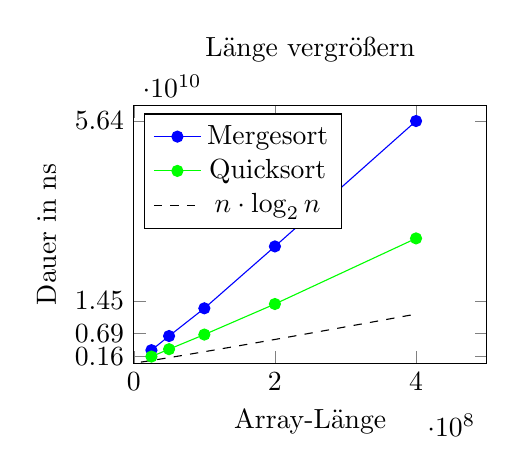
\begin{tikzpicture}
        \begin{axis}[
                title style={yshift=1.5ex},
                width=0.5\textwidth,
                height=0.4\textwidth,
                xlabel={Array-Länge},
                ylabel={Dauer in ns},
                title={Länge vergrößern},
                xmin=0, xmax=5 * 10^8,
                ymin=0*10^6, ymax=6*10^10,
                grid style=dashed,
                legend pos=north west,
                ytick={1609541400,6854920900,14495472700,56441153000},
                % xtick={2^21,2^23,2^24,2^25},
                % xticklabels={$2^{21}$, $2^{23}$, $2^{24}$, $2^{25}$},
                % scaled x ticks=false,
                % scaled y ticks=false,
            ]
            \MergesortMesswerte
            \QuicksortMesswerte
            % n*log2(n)
            \addplot[black, dashed,domain=1e7:4e8, samples=100] {x*log2(x)};
            \addlegendentry{$n \cdot \log_2 n$}
            % % n
            % \addplot[red, dashed,domain=1e7:4e8, samples=100] {x};
            % \addlegendentry{$n$}
            % % log2(n)
            % \addplot[green, domain=1e7:4e8, samples=100] {log2(x)};
            % \addlegendentry{$\log_2 n$}
        \end{axis}
    \end{tikzpicture}%
}

\newcommand{\GrundlegendeLaufzeitenAbhaengigVonDerArraygroesseDiagrammB}{%
    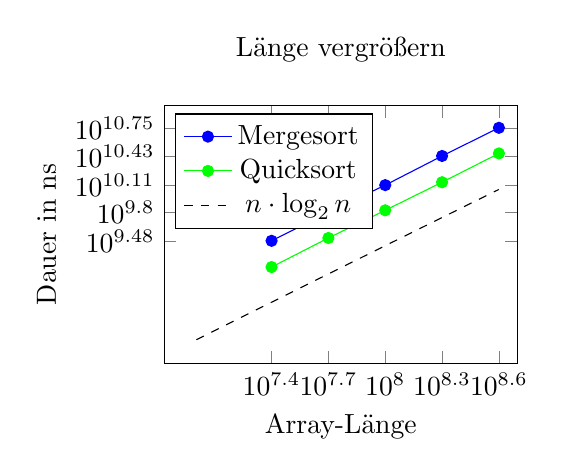
\begin{tikzpicture}
        \begin{axis}[
                title style={yshift=1.5ex},
                width=0.5\textwidth,
                height=0.4\textwidth,
                xlabel={Array-Länge},
                ylabel={Dauer in ns},
                title={Länge vergrößern},
                xmin=0, xmax=5 * 10^8,
                ymin=0*10^6, ymax=1*10^11,
                grid style=dashed,
                legend pos=north west,
                xmode=log,
                log basis x=10,
                xtick=data,
                ymode=log,
                log basis y=10,
                ytick=data,
                % xtick={2^21,2^23,2^24,2^25},
                % xticklabels={$2^{21}$, $2^{23}$, $2^{24}$, $2^{25}$},
                % scaled x ticks=false,
                % scaled y ticks=false,
            ]
            \MergesortMesswerte
            \QuicksortMesswerte
            % n*log2(n)
            \addplot[black, dashed,domain=1e7:4e8, samples=100] {x*log2(x)};
            \addlegendentry{$n \cdot \log_2 n$}
        \end{axis}
    \end{tikzpicture}%
}


% Definiere Variablen
% \newcommand{\Messziel}{Messziel}

% % ----------------------
% % 4. Ergebnisse und Analyse
% % ----------------------
% \newpage
% \chapter{Ergebnisse und Analyse}
% \paragraph{Hinweis zum Umfang der Darstellung}
% \section{Grundlegende Laufzeiten abhängig von der Arraygröße}
% \subsection{Messziel} % Einleitung
% \subsection{Erwartung}
% \subsection{Diagramm}
% \subsection{Analyse und Interpretation}
% \newpage
% \section{Einfluss des Listentyps} % Listentyps: Zufall, Sortiert, InvertiertSortiert, FastSortiert, Dupliziert
% \subsection{Messziel} % Einleitung
% \subsection{Erwartung}
% \subsection{Diagramm}
% \subsection{Analyse und Interpretation}
% \newpage
% \section{Einfluss der Arraygröße im Detail}
% \subsection{Messziel} % Einleitung
% \subsection{Erwartung}
% \subsection{Diagramm}
% \subsection{Analyse und Interpretation}
% \newpage
% \section{Tiefenbasierte Thread-Erzeugung}
% \subsection{Messziel} % Einleitung
% \subsection{Erwartung}
% \subsection{Diagramm}
% \subsection{Analyse und Interpretation}
% \newpage
% \section{Workerthreads}
% \subsection{Messziel} % Einleitung
% \subsection{Erwartung}
% \subsection{Diagramm}
% \subsection{Analyse und Interpretation}
% \newpage
% \section{Vergleich der Threading-Methoden}
% \subsection{Messziel} % Einleitung
% \subsection{Erwartung}
% \subsection{Diagramm}
% \subsection{Analyse und Interpretation}
% \newpage
% \section{Einfluss des Datentyps der Liste} % Listenart: int, string
% \subsection{Messziel} % Einleitung
% \subsection{Erwartung}
% \subsection{Diagramm}
% \subsection{Analyse und Interpretation}
% % \section{Debug Vs Release}

% % ----------------------
% % 4. Ergebnisse und Analyse
% % ----------------------
% \chapter{Ergebnisse und Analyse}
% \paragraph{Hinweis zum Umfang der Darstellung}
\newcommand{\HinweisZumUmfangDerDarstellung}{
    Alle beschriebenen Messungen wurden vollständig durchgeführt und die
    entsprechenden Rohdaten liegen vor. Aufgrund des begrenzten zeitlichen
    Rahmens dieser Bachelorarbeit wird jedoch auf eine vollständige grafische
    Darstellung sowie eine detaillierte Analyse aller Messreihen verzichtet.
    Stattdessen werden im Folgenden ausgewählte, repräsentative Messungen
    dargestellt und analysiert, da diese ausreichend sind, um die theoretisch
    erwarteten Laufzeiteigenschaften der untersuchten Algorithmen zu bestätigen.
    Weitere Messdaten würden keine zusätzlichen inhaltlichen Erkenntnisse liefern,
    sondern lediglich bereits beobachtete Effekte wiederholen.}
% \section{Grundlegende Laufzeiten abhängig von der Arraygröße}

% \subsection{Messziel} % Einleitung
\newcommand{\GrundlegendeLaufzeitenAbhaengigVonDerArraygroesseMessziel}{
    Das Messziel besteht darin, die Abhängigkeit des seriellen Algorithmus von der Arraygröße grafisch darzustellen.
    Dadurch können diese Ergebnisse später mit den nicht-seriellen Varianten verglichen werden.
    Gleichzeitig dient dies als einfacher Einstieg in das Thema.
}

% \subsection{Erwartung}
\newcommand{\GrundlegendeLaufzeitenAbhaengigVonDerArraygroesseErwartung}{
    Da die durchschnittliche Laufzeit \(O(n \log n)\) beträgt, erwarte ich eine logarithmische Laufzeiterhöhung bei wachsender Arraygröße.
}
% \subsection{Diagramm}
\newcommand{\GrundlegendeLaufzeitenAbhaengigVonDerArraygroesseDiagramm}{
    \GrundlegendeLaufzeitenAbhaengigVonDerArraygroesseDiagrammA
    \GrundlegendeLaufzeitenAbhaengigVonDerArraygroesseDiagrammB
    \newline
    \GrundlegendeLaufzeitenAbhaengigVonDerArraygroesseDiagrammC
}

% \subsection{Analyse und Interpretation}
\newcommand{\GrundlegendeLaufzeitenAbhaengigVonDerArraygroesseAnalyse}{
    In den ersten zwei Diagrammen ist die Veränderung der Laufzeit zu sehen, wenn die Listengröße fünfmal verdoppelt wird und bei \(2.5 \cdot 10^7\) startet.
    Beim zweiten Diagramm sind die Achsen logarithmisch dargestellt, da dies die Darstellung und den Vergleich der Laufzeiten erleichtert.
    \newline
    Unter diesen beiden Diagrammen befindet sich ein drittes Diagramm, in dem die gemessenen Laufzeiten ebenfalls logarithmisch dargestellt sind und der Größenbereich von \(1\) bis \(800\,000\) betrachtet wird.
    \newline
    Anhand dieser Diagramme ist deutlich erkennbar, dass sowohl Mergesort als auch Quicksort tatsächlich eine Laufzeit von
    \(O(n \log n)\) besitzen.
    \newline
    Zudem ist erkennbar, dass Mergesort etwa doppelt so lange benötigt wie Quicksort und dass Quicksort näherungsweise eine Laufzeit von
    \(2 \cdot n \log_2(n)\) aufweist.
    Aus diesen Beobachtungen lässt sich ableiten, dass der Partitionierungsschritt eine Laufzeit von etwa \(2n\) besitzt, während der Merge-Schritt näherungsweise eine Laufzeit von \(4n\) aufweist.
    Zur Vereinfachung der Betrachtung wird jedoch bei beiden Algorithmen weiterhin von \(n\) ausgegangen.
    \newline
    Da eine lineare Laufzeit auf einen Blick leichter zu interpretieren ist, wurde zusätzlich die Funktion \(32n\) eingezeichnet.
    Anhand dieser Funktion ist erkennbar, dass sie im untersuchten Zahlenbereich von \(1\) bis \(4 \cdot 10^8\) teilweise sogar eine genauere Abschätzung liefert als \(n \log_2(n)\).
    Daraus folgt, dass von einer gerundeten Mindestlaufzeit von \(32n\) ausgegangen werden kann.
    \newline
    Abschließend ist anzumerken, dass alle Messungen mit einer Laufzeit von kleiner oder gleich \(10^4\,\text{ns}\) aufgrund der Messtoleranz nur eine eingeschränkte Aussagekraft besitzen.
    Zwar kann mit \texttt{chrono} auf eine Auflösung von \(100\,\text{ns}\) genau gemessen werden, dennoch verbleiben natürliche Schwankungen, die insbesondere im Bereich von \(10^4\,\text{ns}\) einen erheblichen Einfluss auf die Messergebnisse haben.
}

% \section{Einfluss des Listentyps} % Listentyps: Zufall, Sortiert, InvertiertSortiert, FastSortiert, Dupliziert
% \subsection{Messziel} % Einleitung
\newcommand{\EinflussDesListentypsMessziel}{
    Der Listentyp ist relevant, da es bei Quicksort einen Best-Case sowie einen Worst-Case gibt.
    Diese hängen vom Inhalt der zu sortierenden Liste ab und somit auch vom Listentyp.
    Gleichzeitig dient diese Messung der Vollständigkeit, damit die Laufzeiten auch mit anderen,
    nicht von mir implementierten Sortieralgorithmen gut vergleichbar sind.
    Auch hierbei werden zunächst nur die seriellen Laufzeiten der Algorithmen gemessen.
    Zur Vollständigkeit werden hierbei zusätzlich weitere Listentypen außer zufällig und sortiert betrachtet.
}
% \subsection{Erwartung}
\newcommand{\EinflussDesListentypsErwartung}{
    Ich erwarte, dass der Listentyp bei Mergesort nahezu keinen Einfluss hat und somit nur sehr geringe Laufzeitänderungen zu beobachten sind.
    Bei Quicksort erwarte ich hingegen bei einer sortierten Liste exakt den Best-Case,
    da als Pivotelement jeweils das mittlere Element gewählt wird.
    Ebenso erwarte ich, dass bei Quicksort bei Wahl des jeweils ganz rechten Elements als Pivotelement
    bei einer sortierten Liste der Worst-Case eintritt.
}
% \subsection{Diagramm}
\newcommand{\EinflussDesListentypsDiagramm}{
    \EinflussDesListentypsDiagrammA
    \newline
    \EinflussDesListentypsDiagrammB
    \newline
    \EinflussDesListentypsDiagrammC
}
% \subsection{Analyse und Interpretation}
\newcommand{\EinflussDesListentypsAnalyse}{
    Die gemessenen Daten zeigen deutlich, dass der Best Case von Quicksort in der Praxis besser als \(n \log_2(n)\) ausfällt. Dies ist darauf zurückzuführen, dass die Messungen in der Release-Version mit aktivierten Compiler-Optimierungen durchgeführt wurden.
    In der Debug-Version (ohne Compiler-Optimierungen) wurde bei einem sortierten Array der Größe von 400 Millionen Elementen hingegen eine Laufzeit von 14~s für Quicksort gemessen, welche wiederum oberhalb der erwarteten Laufzeit von \(n \log_2(n)\) liegt.
    Die Messungen zeigen außerdem, dass sortierte, invertiert sortierte sowie fastsortierte Arrays nahezu identische Laufzeiten erzeugen. Die entsprechenden Kurven würden nahezu aufeinanderliegen, weshalb auf eine separate grafische Darstellung dieser Listentypen zugunsten der Übersichtlichkeit verzichtet wurde.
}

% \section{Tiefenbasierte Thread-Erzeugung}
% \subsection{Messziel} % Einleitung
% \subsection{Erwartung}
% \subsection{Diagramm}
% \subsection{Analyse und Interpretation}

% \section{Tiefenbasierte Thread-Erzeugung}
% \subsection{Messziel} % Einleitung
\newcommand{\TiefenbasierteThreadErzeugungMessziel}{
    Hier messen wir die rekursive Variante, die einen der beiden rekursiven Selbstaufrufe in einem neuen Thread ausführt.
    Dabei gibt es jedoch ein Limit, da jeder Thread selbst Speicher benötigt und der RAM nicht unendlich groß ist.
    Hierbei soll gemessen werden, welchen Performance-Unterschied eine höhere Anzahl an Threads bewirkt.
}
% \subsection{Erwartung}
\newcommand{\TiefenbasierteThreadErzeugungErwartung}{
    Ich erwarte einen theoretisch linearen Performance-Zuwachs, solange kein Hardware-Limit dazwischenkommt.
    Zudem erwarte ich in dieser Variante, dass Mergesort besser skaliert als Quicksort,
    da Quicksort die Liste nicht exakt in der Mitte teilt, sondern nur dies theoretisch im Durchschnitt tut.
    Der Best Case von Quicksort sollte jedoch immer noch wesentlich besser sein als der von Mergesort,
    da Quicksort in diesem Fall die Liste immer perfekt in der Mitte teilt.
}
% \subsection{Diagramm}
\newcommand{\TiefenbasierteThreadErzeugungDiagramm}{
    \TiefenbasierteThreadErzeugungDiagrammA
}
% \subsection{Analyse und Interpretation}
\newcommand{\TiefenbasierteThreadErzeugungAnalyse}{
    Entgegen der ursprünglichen Erwartung konnte kein signifikanter Unterschied zwischen einer vollständig sortierten und einer nahezu sortierten Liste festgestellt werden.
    Dieses Verhalten ist vermutlich auf Compiler-Optimierungen zurückzuführen sowie darauf, dass in der Implementierung nicht systematisch ein besonders ungünstiges Pivot-Element gewählt wurde.
    \newline
    Deutliche Performance-Verbesserungen sind jedoch in allen Bereichen messbar, wie theoretisch zu erwarten war.
    Für ein unsortiertes Array der Größe \(400 \, \text{Mio.}\) zeigt sich, dass Mergesort mit 16 Threads lediglich etwa 16~\% der Laufzeit der seriellen Variante benötigt, während Quicksort 26~\% erreicht.
    Die Laufzeit von Mergesort wächst dabei sehr konstant, während Quicksort im Durchschnitt ebenfalls eine konsistente Steigerung der Laufzeit zeigt, jedoch stärker schwankt.
    Aufgrund der weiterhin bestehenden Worst-Case-Komplexität von Quicksort ist für sehr große Arrays die Verwendung von Mergesort eindeutig zu bevorzugen.
    \newline
    Bemerkenswert ist, dass die 16-Thread-Variante von Quicksort nur rund 85~\% der Laufzeit von Mergesort erreicht, wodurch Mergesort insgesamt überlegen bleibt.
    Außerdem wird deutlich, dass Performance-Vorteile erst ab einer Array-Größe von etwa 20.000 Elementen auftreten, was auf den Overhead der Thread-Erzeugung zurückzuführen ist.
    \newline
    Zusammenfassend lässt sich festhalten, dass Mergesort insbesondere dann die bessere Wahl ist, wenn die Worst-Case-Laufzeit von Quicksort nicht tolerierbar ist.
    Für typische, nicht degenerierte Listen zeigt Quicksort im Durchschnitt eine konstante und effiziente Leistungssteigerung, wobei die Best- und Worst-Case-Laufzeiten stets berücksichtigt werden sollten.
}

% \section{Workerthreads}
% \subsection{Messziel} % Einleitung
% \subsection{Erwartung}
% \subsection{Diagramm}
% \subsection{Analyse und Interpretation}

% \section{Workerthreads}
% \subsection{Messziel} % Einleitung
\newcommand{\WorkerthreadsMessziel}{
    Hier messen wir die Worker-Thread-Variante nach einem Work-Stealing-Ansatz mit einer unterstützten
    Thread-Anzahl von \(N\), wobei Quicksort als iterative Version umgesetzt ist.
    Zusätzlich messen wir die Zeit, die die Threads für ihre Initialisierung benötigen mit.
    Da in unserem Fall die Worker-Threads nach dem Sortieren nicht wiederverwendet werden,
    ist diese Messung nicht vollständig fair.
    \newline
    In der Praxis würde man die Threads weiterverwenden, wodurch dieser Overhead geringer ausfallen würde.
    Bei der Worker-Thread-Variante wurde außerdem eine Mindestgröße von 4.000 Elementen für neue Threads eingeführt.
    Dies geschieht aus dem schlichten Grund, dass sich andernfalls kein Performance-Vorteil durch zusätzliche Threads ergibt,
    da der entstehende Overhead sonst zu groß ist.
}
% \subsection{Erwartung}
\newcommand{\WorkerthreadsErwartung}{
    Es wird erwartet, dass Mergesort in der Worker-Thread-Variante schlechtere Ergebnisse erzielt als bei der tiefenbasierten Thread-Erzeugung.
    Dies ist darauf zurückzuführen, dass sich die Arbeit bei Mergesort in dieser Variante nur selten gleichmäßig auf die verfügbaren Threads verteilt.
    \newline
    Ebenso wird erwartet, dass der Best-Case von Quicksort im Vergleich zur tiefenbasierten Variante schlechter ausfällt, da auch hier keine optimale Arbeitsaufteilung erreicht wird.
    Für den Average-Case von Quicksort wird hingegen eine bessere Performance erwartet, da der Work-Stealing-Ansatz eine gleichmäßigere Lastverteilung über mehrere Threads ermöglicht.
}
% \subsection{Diagramm}
\newcommand{\WorkerthreadsDiagramm}{
    \WorkerthreadsDiagrammA
}
% \subsection{Analyse und Interpretation}
\newcommand{\WorkerthreadsAnalyse}{
    Die Messergebnisse bestätigen die zuvor formulierten Erwartungen.
    Zu beachten ist, dass die Mergesort-Worker-Thread-Variante erst ab einer Array-Größe von 64.000 Elementen alle 16 Threads nutzt.
    Dies liegt am Mindestlimit von 4.000 Elementen für die Erzeugung neuer Threads.
}
